\documentclass[tikz, border=3pt]{standalone}
\usepackage{tikz}
\usetikzlibrary{
    positioning, 
    arrows.meta, 
    backgrounds, 
    decorations.pathreplacing, 
    decorations.pathmorphing, 
    calc, 
    fit
}

\begin{document}
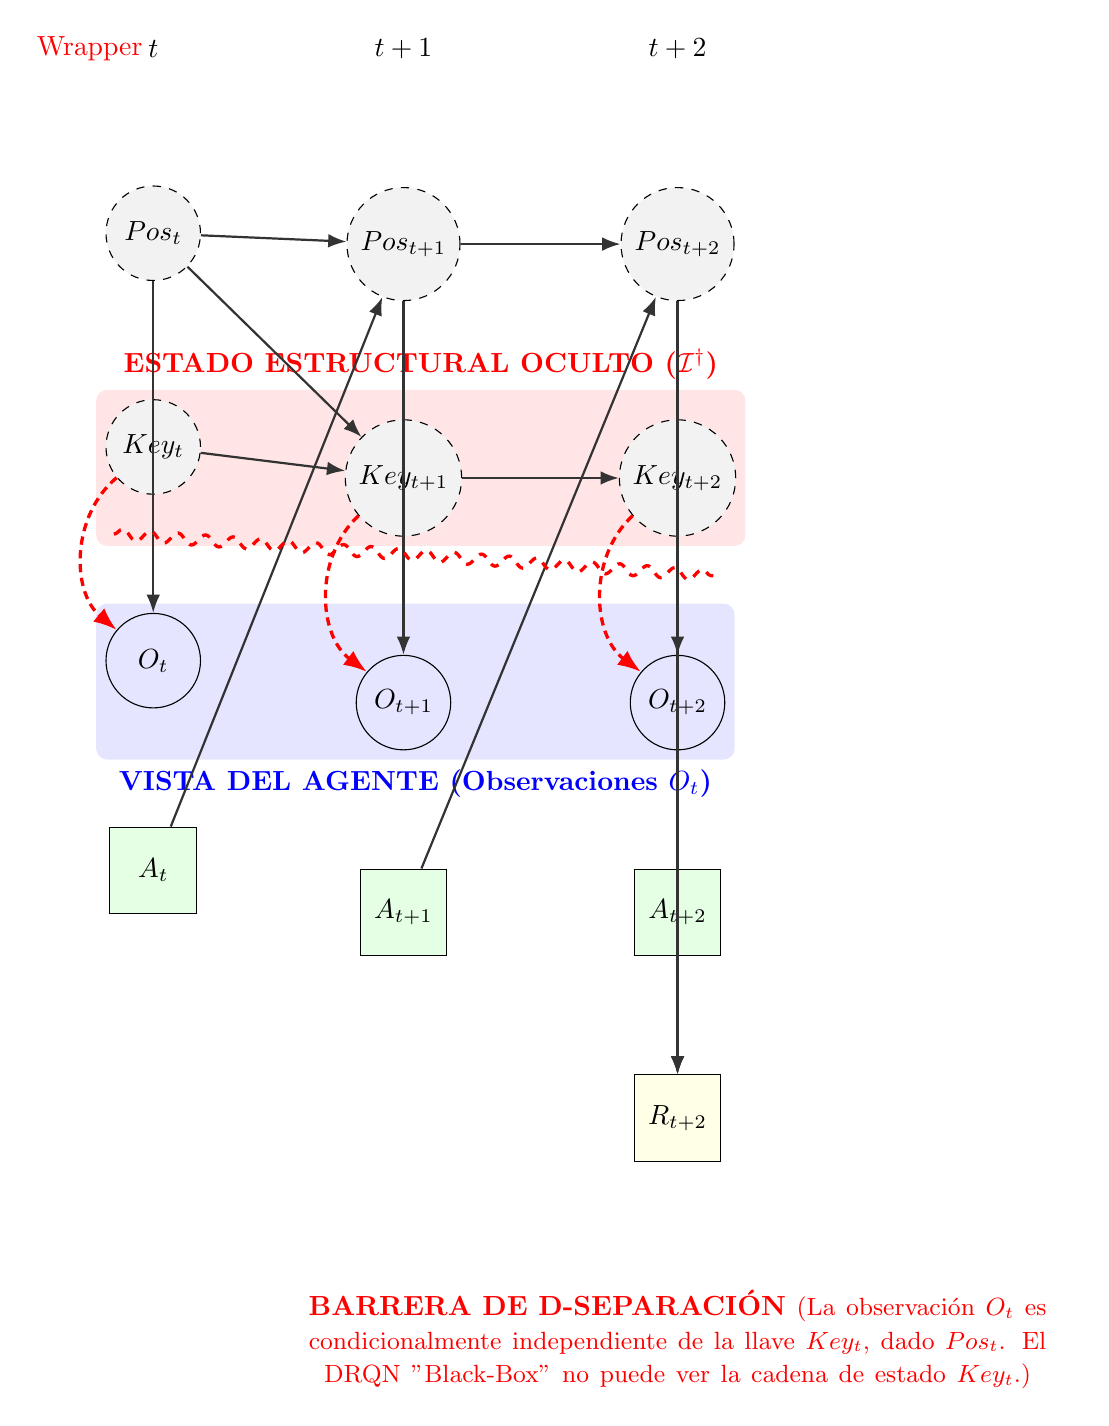
\begin{tikzpicture}[
    node distance=1.5cm and 2.5cm,
    % Estilos de Nodos
    latent/.style={circle, draw=black, dashed, fill=gray!10, minimum size=1.2cm},
    observed/.style={circle, draw=black, fill=blue!10, minimum size=1.2cm},
    action/.style={rectangle, draw=black, fill=green!10, minimum size=1.1cm},
    reward/.style={rectangle, draw=black, fill=yellow!10, minimum size=1.1cm},
    % Estilos de Flechas
    arrow/.style={-Latex, thick, draw=black!80},
    info_arrow/.style={-Latex, thick, draw=red, densely dashed, very thick} % La flecha del sesgo
]

% --- Columnas de Tiempo ---
\node (t) {$t$};
\node (t1) [right=of t, node distance=4.5cm] {$t+1$};
\node (t2) [right=of t1, node distance=4.5cm] {$t+2$};

% === TIEMPO t (Ej: Recoger Llave) ===
\node[latent] (pos_t) [below=of t, node distance=1.5cm] {$Pos_t$};
\node[latent] (key_t) [below=of pos_t, node distance=1.5cm] {$Key_t$};
\node[observed] (obs_t) [below=of key_t, node distance=2cm] {$O_t$};
\node[action] (act_t) [below=of obs_t, node distance=1.5cm] {$A_t$};

% === TIEMPO t+1 (Ej: Pasillo Ruidoso) ===
\node[latent] (pos_t1) [below=of t1, node distance=1.5cm] {$Pos_{t+1}$};
\node[latent] (key_t1) [below=of pos_t1, node distance=1.5cm] {$Key_{t+1}$};
\node[observed] (obs_t1) [below=of key_t1, node distance=2cm] {$O_{t+1}$};
\node[action] (act_t1) [below=of obs_t1, node distance=1.5cm] {$A_{t+1}$};

% === TIEMPO t+2 (Ej: Decisión en la Puerta) ===
\node[latent] (pos_t2) [below=of t2, node distance=1.5cm] {$Pos_{t+2}$};
\node[latent] (key_t2) [below=of pos_t2, node distance=1.5cm] {$Key_{t+2}$};
\node[observed] (obs_t2) [below=of key_t2, node distance=2cm] {$O_{t+2}$};
\node[action] (act_t2) [below=of obs_t2, node distance=1.5cm] {$A_{t+2}$};
\node[reward] (rew_t2) [below=of act_t2, node distance=1.5cm] {$R_{t+2}$};


% --- Flechas de Transición (S_t, A_t) -> S_{t+1} ---
\draw[arrow] (pos_t) -- (pos_t1);
\draw[arrow] (act_t) -- (pos_t1);
\draw[arrow] (key_t) -- (key_t1);
\draw[arrow] (pos_t) -- (key_t1); % La posición (Pos_t) en la llave afecta Key_{t+1}

\draw[arrow] (pos_t1) -- (pos_t2);
\draw[arrow] (act_t1) -- (pos_t2);
\draw[arrow] (key_t1) -- (key_t2); % La memoria de la llave se propaga

% --- Flechas de Emisión (S_t -> O_t) ---
\draw[arrow] (pos_t) -- (obs_t);
\draw[arrow] (pos_t1) -- (obs_t1);
\draw[arrow] (pos_t2) -- (obs_t2);
% ¡NOTA LA AUSENCIA DE FLECHAS DE Key_t a O_t!

% --- Flechas de Recompensa (S_t, A_t -> R_t) ---
% La recompensa en t+2 depende de la acción, la posición Y la llave
\draw[arrow] (pos_t2) -- (rew_t2);
\draw[arrow] (key_t2) -- (rew_t2);
\draw[arrow] (act_t2) -- (rew_t2);

% --- VISUALIZACIÓN DE D-SEPARACIÓN ---
\begin{pgfonlayer}{background}
    % Capa 1: Estado Estructural Oculto (Lo que el agente NECESITA)
    \node [fill=red!10, rounded corners,
           fit=(key_t) (key_t1) (key_t2), 
           label={[red, font=\bfseries]above:ESTADO ESTRUCTURAL OCULTO ($\mathcal{I}^\dagger$)}] {};
           
    % Capa 2: Información del Agente (Lo que el agente VE)
    \node [fill=blue!10, rounded corners,
           fit=(obs_t) (obs_t1) (obs_t2), 
           label={[blue, font=\bfseries]below:VISTA DEL AGENTE (Observaciones $O_t$)}] {};
\end{pgfonlayer}

% --- Línea de D-Separación (sin texto) ---
\draw [red, dashed, very thick, decoration={snake, segment length=10pt, amplitude=2pt}, decorate] 
    ($(key_t.south)+(-0.5, -0.5)$) -- ($(key_t2.south)+(0.5, -0.5)$);

% --- Flechas del Wrapper (La Solución) ---
\draw[info_arrow] (key_t) to [bend right=50] (obs_t) node [pos=0.8, left, text=red] {Wrapper};
\draw[info_arrow] (key_t1) to [bend right=50] (obs_t1);
\draw[info_arrow] (key_t2) to [bend right=50] (obs_t2);

% --- Texto de D-Separación (Movido al final) ---
\node [text=red, font=\bfseries, text width=10cm, align=center,
       below=of rew_t2, node distance=2.5cm] % <-- MOVIDO AQUÍ
    {BARRERA DE D-SEPARACIÓN
    \normalfont \small (La observación $O_t$ es condicionalmente independiente de la llave $Key_t$, dado $Pos_t$. El DRQN "Black-Box" no puede ver la cadena de estado $Key_t$.)};

\end{tikzpicture}
\end{document}